\documentclass[acmtog]{acmart}
\usepackage{graphicx}
\usepackage{subfigure}
\usepackage{natbib}
\usepackage{listings}
\usepackage{bm}
\usepackage{amsmath}

\definecolor{blve}{rgb}{0.3372549 , 0.61176471, 0.83921569}
\definecolor{gr33n}{rgb}{0.29019608, 0.7372549, 0.64705882}
\makeatletter
\lst@InstallKeywords k{class}{classstyle}\slshape{classstyle}{}ld
\makeatother
\lstset{language=C++,
	basicstyle=\ttfamily,
	keywordstyle=\color{blve}\ttfamily,
	stringstyle=\color{red}\ttfamily,
	commentstyle=\color{magenta}\ttfamily,
	morecomment=[l][\color{magenta}]{\#},
	classstyle = \bfseries\color{gr33n}, 
	tabsize=2
}
\lstset{basicstyle=\ttfamily}

% Title portion
\title{Assignment 3: {Ray Tracing Basics}} 

\author{Name:\quad Bingnan Li  \\ student number:\ 2020533092
\\email:\quad libn@shanghaitech.edu.cn}

% Document starts
\begin{document}
\maketitle

\vspace*{2 ex}

\section{Introduction}
\begin{enumerate}
	\item Generate ray from camera
	\item Ray geometry intersection
	\item Phong lighting at intersection points
	\item Soft shadow
	\item Anti-aliasing via super-resolution
	\item Texture mapping
	\item Normal and displacement texture
	\item Advanced anti-aliasing via rotation
\end{enumerate}

\section{Implementation Details}
\begin{enumerate}
	\setlength\parindent{2em}
	\item Generate ray from camera
	\par Once we get coordinate of pixel $(dx,\ dy)$, we can calculate the corresponding coordinate in world space by the following procedure:
	\begin{align*}
		2\times\frac{dx}{x_{resolution}} - 1 &= \frac{x_{coef}}{AspectRatio\times focal\_length\times\tan(fov/2)}\\
		2\times\frac{dy}{y_{resolution}} - 1 &= \frac{y_{coef}}{focal\_length\times\tan(fov/2)}
	\end{align*}
	Then the world coordinate is 
	\[P =  {\bf forward} + x_coef\times {\bf right} + y_coef \times {\bf up}\]
	And the direction of generated ray is 
	\[{\bf ray\_dir}=normalize(P-P_{camera})\]
	Thus, the expression of ray is 
	\[r(t)=P_{camera}+t\times {\bf ray\_dir}\]
	\item Ray geometry intersection
	\begin{enumerate}
		\setlength\parindent{2em}
		\item Triangle intersection:
		\par Assume that ray is $r(t)=o+t{\bf d}$ and barycentric coordinate of intersection point is $(b_1,b_2, 1-b_1-b_2)$, then we have
		\begin{align*}
			o+t{\bf d}&=(1-b_1-b_2)p_0+b_1p_1+b_2p_2\\
			o+t{\bf d}&=p_0+(p_1-p_0)b_1+(p_2-p_0)b_2
		\end{align*}
		Let $s=o-p_0,\ e_1=p_1-p_0,\ e_2=p_2-p_0$, we can rewrite the equation as following form:
		\[[-d,e_1,e_2]\begin{bmatrix}
			t\\ b_1\\ b_2
		\end{bmatrix}=s\]
		Then, by Cramer's rule, we have
		\[\begin{bmatrix}
		t\\ b_1\\ b_2
	\end{bmatrix}=\frac{1}{|-d\ e_1\ e_2|}\begin{bmatrix}
		|&s & e_1 & e_2&|\\
		|&-d & s & e_2&|\\
		|&-d & e_1 & s&|
	\end{bmatrix}\]
	Then let $s_1=d\times e_2,\ s_2=s\times e_1$, we have 
	\begin{align*}
		\begin{bmatrix}
			t\\ b_1\\ b_2
		\end{bmatrix}=\frac{1}{s_1\cdot e_1}\begin{bmatrix}
			s_2\cdot e_2\\
			s_1\cdot s\\
			s_2\cdot d
		\end{bmatrix}
	\end{align*}
	Once we get $b_1$ and $b_2$, we can check whether $b_1\geq 0,b_2\geq 0$ and $b_1+b_2\leq 1$, if they do, then ray intersects with triangle.
	\item Rectangle intersection:
	\par The known knowledge of rectangle is its geometrical center $p_0$, length $x$, width $y$, normal vector ${\bf n}$ and tangent vector ${\bf t}$.
	\par Based on that, we can firstly calculate cotangent vector ${\bf c}$ by cross product:
	\[{\bf c} = normalize({\bf n}\times {\bf t})\]
	Then we calculate the intersection point $p$
	\begin{align*}
		&n(o+t{\bf d}-p_0)=0\\
		&t=\frac{n\cdot p_0-n\cdot o}{n\cdot {\bf d}}\\
		&p=o+t{\bf d}
	\end{align*}
	Then we check whether
	\begin{align*}
		{\bf pp_0}\cdot {\bf t}\leq \frac{x}{2}\\
		{\bf pp_0}\cdot {\bf c}\leq \frac{y}{2}
	\end{align*}
	if they do, then ray intersects with rectangle;
	\item Ellipsoid intersection:
	\par The know knowledge of ellipsoid is
	\begin{itemize}
		\item C  = Center of the ellipsoid in world space
		\item ${\bf a}$ = First ellipsoid axis vector (along local x-axis)
		\item ${\bf b}$ = Second ellipsoid axis vector (along local y-axis)
		\item ${\bf c}$ = Third ellipsoid axis vector (along local z-axis)
		
		\item $L_0$ = Point on the line in world space
		\item ${\bf v}$ = Vector that defines the line direction in world space
		
		\item P = Point on the surface of a unit radius sphere centered in the origin
	\end{itemize}
	\par First, we need to transfer ellipsoid into a standard unit sphere. In order to do that, we need to construct the following three matrices:
	\begin{align*}
		T&=
		\begin{bmatrix}
			1 & 0 & 0 & C_x\\
			0 & 1 & 0 & C_y\\
			0 & 0 & 1 & C_z\\
			0 & 0 & 0 & 1
		\end{bmatrix}\\
		R&=
		\begin{bmatrix}
			\hat{a}_x & \hat{b}_x & \hat{c}_x & 0 \\
			\hat{a}_y & \hat{b}_y & \hat{c}_y & 0 \\
			\hat{a}_z & \hat{b}_z & \hat{c}_z & 0 \\
			0 & 0 & 0 & 1
		\end{bmatrix}\\
		S&=
		\begin{bmatrix}
			||a|| & 0 & 0 & 0 \\
			0 & ||b|| & 0 & 0 \\
			0 & 0 & ||c|| & 0 \\
			0 & 0 & 0 & 1
		\end{bmatrix}\\
		M&=TRS
	\end{align*}
	Then we use $M^{-1}$ to transform ray
	\[r'(t)=M^{-1}o+tM^{-1}{\bf d}=o'+t{\bf d'}\]
	Then check if $r'(t)$ intersects with sphere, we can determine whether $r(t)$ intersects with ellipsoid.
	\end{enumerate}
	\item Phong lighting at intersection points and soft shadow
	\par For each intersection point, we construct shadow ray to perform visibility test. The construction process is like: for each light sample, generate new ray from intersection point to light sample. After that, we need to check whether this shadow ray intersects with other geometries between intersection point and light sample. If visibility succeed, then we apply phong lighting model into that point. Once we traverse all sample light, we divided diffuse and specular light result by sample size to get correct value.
	\item Anti-aliasing via super-resolution and rotation\newline
	In order to do that, we generate more than 1 ray from camera at each pixel, then calculate the average value of those rays to be the final value. For rotation, I rotated sample points based on the sample cell center by 26.6 degree.
	\item Texture mapping and normal/displacement texture
	\par We first load texture from disk, then each time we find intersection point, we need to calculate the corresponding u/v value to determine the color of this point based on texture.
	\par In order to get u/v coordinate, we do the following procedure:
	\begin{align*}
		(u,v)=(({{\bf pp_0}\cdot {\bf t}, {\bf pp_0}\cdot {\bf c}}) + 1) / 2 
	\end{align*} 
	\par For normal and displacement texture, we use normal texture color as new normal by the following process: assume normal texture value is $n$, then we need to calculate $\frac{n}{255} \times 2 - 1$ to convert $n$ into range $(0, 1)$, then we transfer $n$ from tangent space into world space with the following matrix
	\[\begin{bmatrix}
		t_x & b_x & n_x & 0\\
		t_y & b_y & n_y & 0\\
		t_z & b_z & n_z & 0\\
		0 & 0 & 0 & 1
	\end{bmatrix}\]
	For displacement texture, we use first get value $h$ of displacement texture at position $u,\ v$, then we calculate $1 - h$ to be the distortion value, and we translate intersection position along normal direction by $1-h$ unit.
\end{enumerate}
\section{Results}
\begin{itemize}
	\item Cornell-box without anti-aliasing:
	\begin{figure}[H]
		\centering
		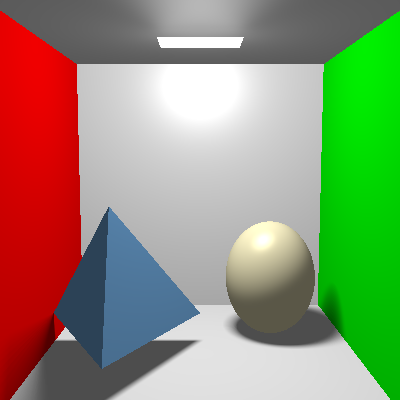
\includegraphics[width=0.45\textwidth]{"/home/lee/Desktop/CG/PA3/report/images/Cornell_box_no_anti_aliasing.png"}
	\end{figure}
	\item Cornell-box with super-resolution(4-ray each pixel):
	\begin{figure}[H]
		\centering
		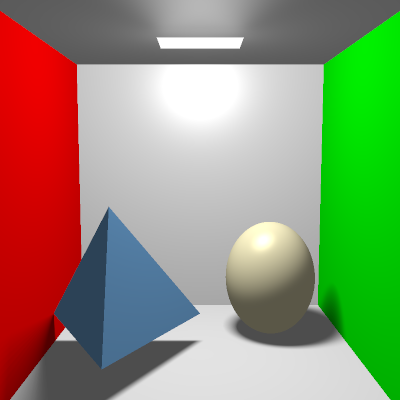
\includegraphics[width=0.45\textwidth]{"/home/lee/Desktop/CG/PA3/report/images/Cornell_box_with_2_super_resolution.png"}
	\end{figure}
	\item Cornell-box with super-resolution(16-ray each pixel)
	\begin{figure}[H]
		\centering
		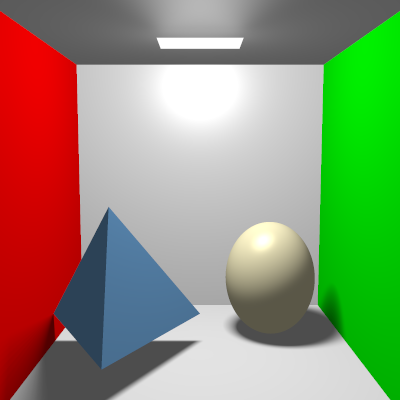
\includegraphics[width=0.45\textwidth]{"/home/lee/Desktop/CG/PA3/report/images/Cornell_box_with_4_super_resolution.png"}
	\end{figure}
	\item Cornell-box with rotation anti-aliasing(4-ray each pixel)
	\begin{figure}[H]
		\centering
		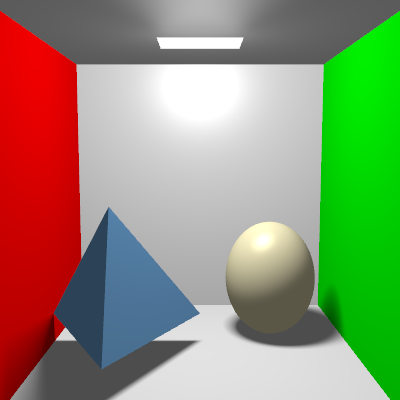
\includegraphics[width=0.45\textwidth]{"/home/lee/Desktop/CG/PA3/report/images/Cornell_box_with_2_sr_rotation.png"}
	\end{figure}
	\item without anti aliasing
	\begin{figure}[H]
		\centering
		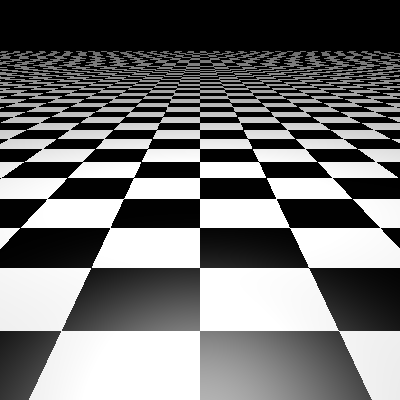
\includegraphics[width=0.45\textwidth]{"/home/lee/Desktop/CG/PA3/report/images/no_anti_aliasing.png"}
	\end{figure}
	\item anti aliasing with super resolution
	\begin{figure}[H]
		\centering
		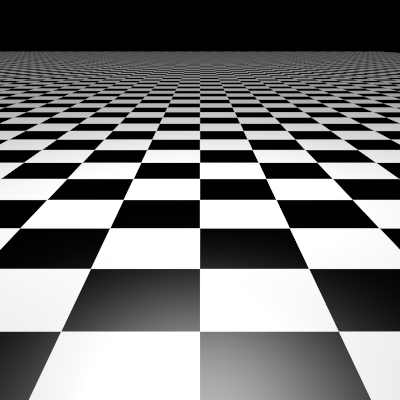
\includegraphics[width=0.45\textwidth]{"/home/lee/Desktop/CG/PA3/report/images/anti_aliasing_with_16_super_sampling.png"}
	\end{figure}
	\item anti aliasing with rotation
	\begin{figure}[H]
		\centering
		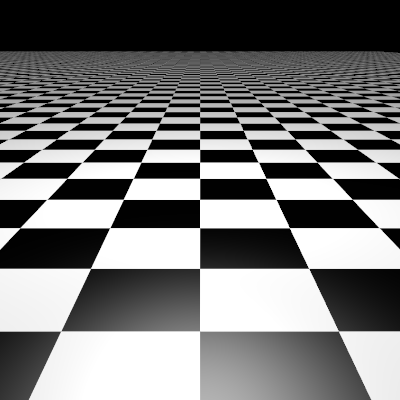
\includegraphics[width=0.45\textwidth]{"/home/lee/Desktop/CG/PA3/report/images/anti_aliasing_with_rotation.png"}
	\end{figure}
	\item anti aliasing with rotation and super resolution
	\begin{figure}[H]
		\centering
		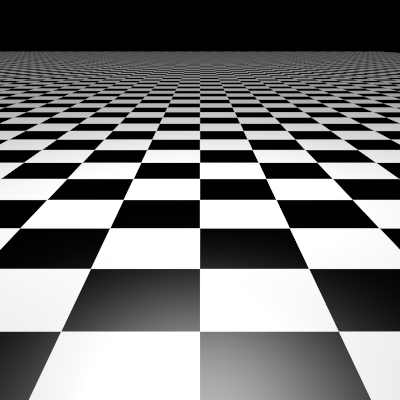
\includegraphics[width=0.45\textwidth]{"/home/lee/Desktop/CG/PA3/report/images/anti_aliasing_with_16_super_sampling.png"}
	\end{figure}
	\item Apply normal texture
	\begin{figure}[H]
		\centering
		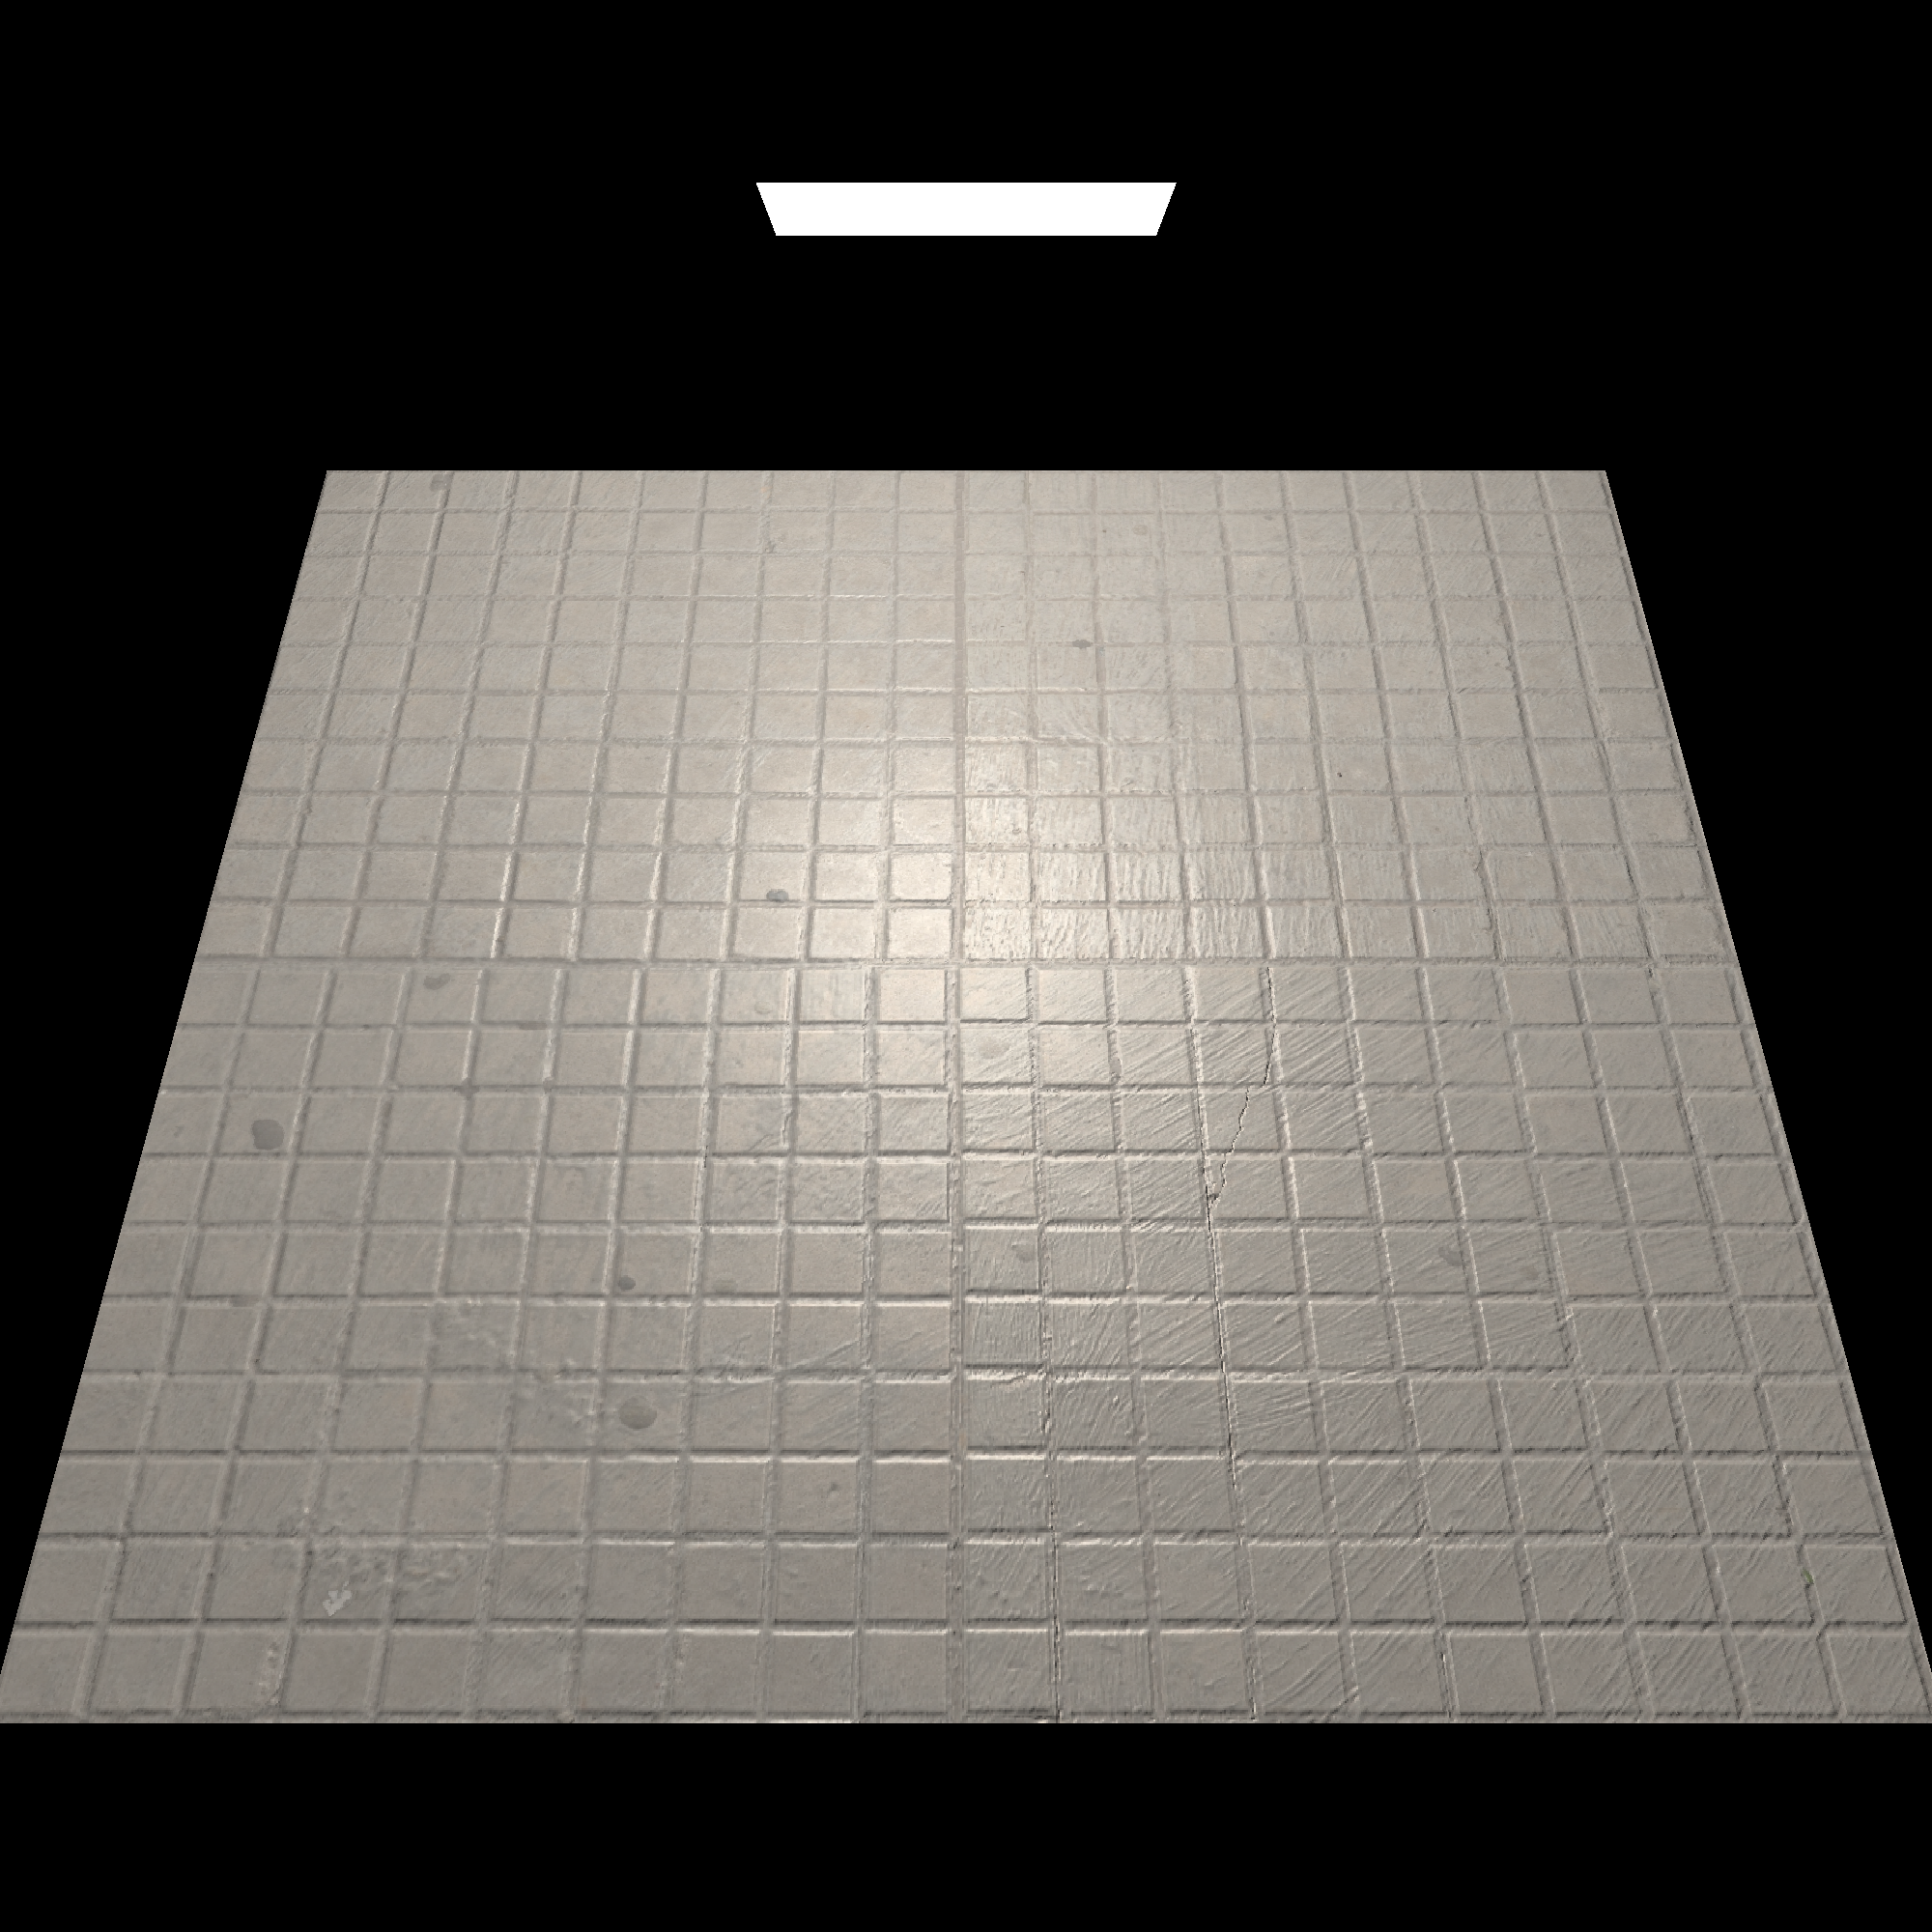
\includegraphics[width=0.45\textwidth]{"/home/lee/Desktop/CG/PA3/report/images/normal.png"}
	\end{figure}
	\item Apply displacement texture
	\begin{figure}[H]
		\centering
		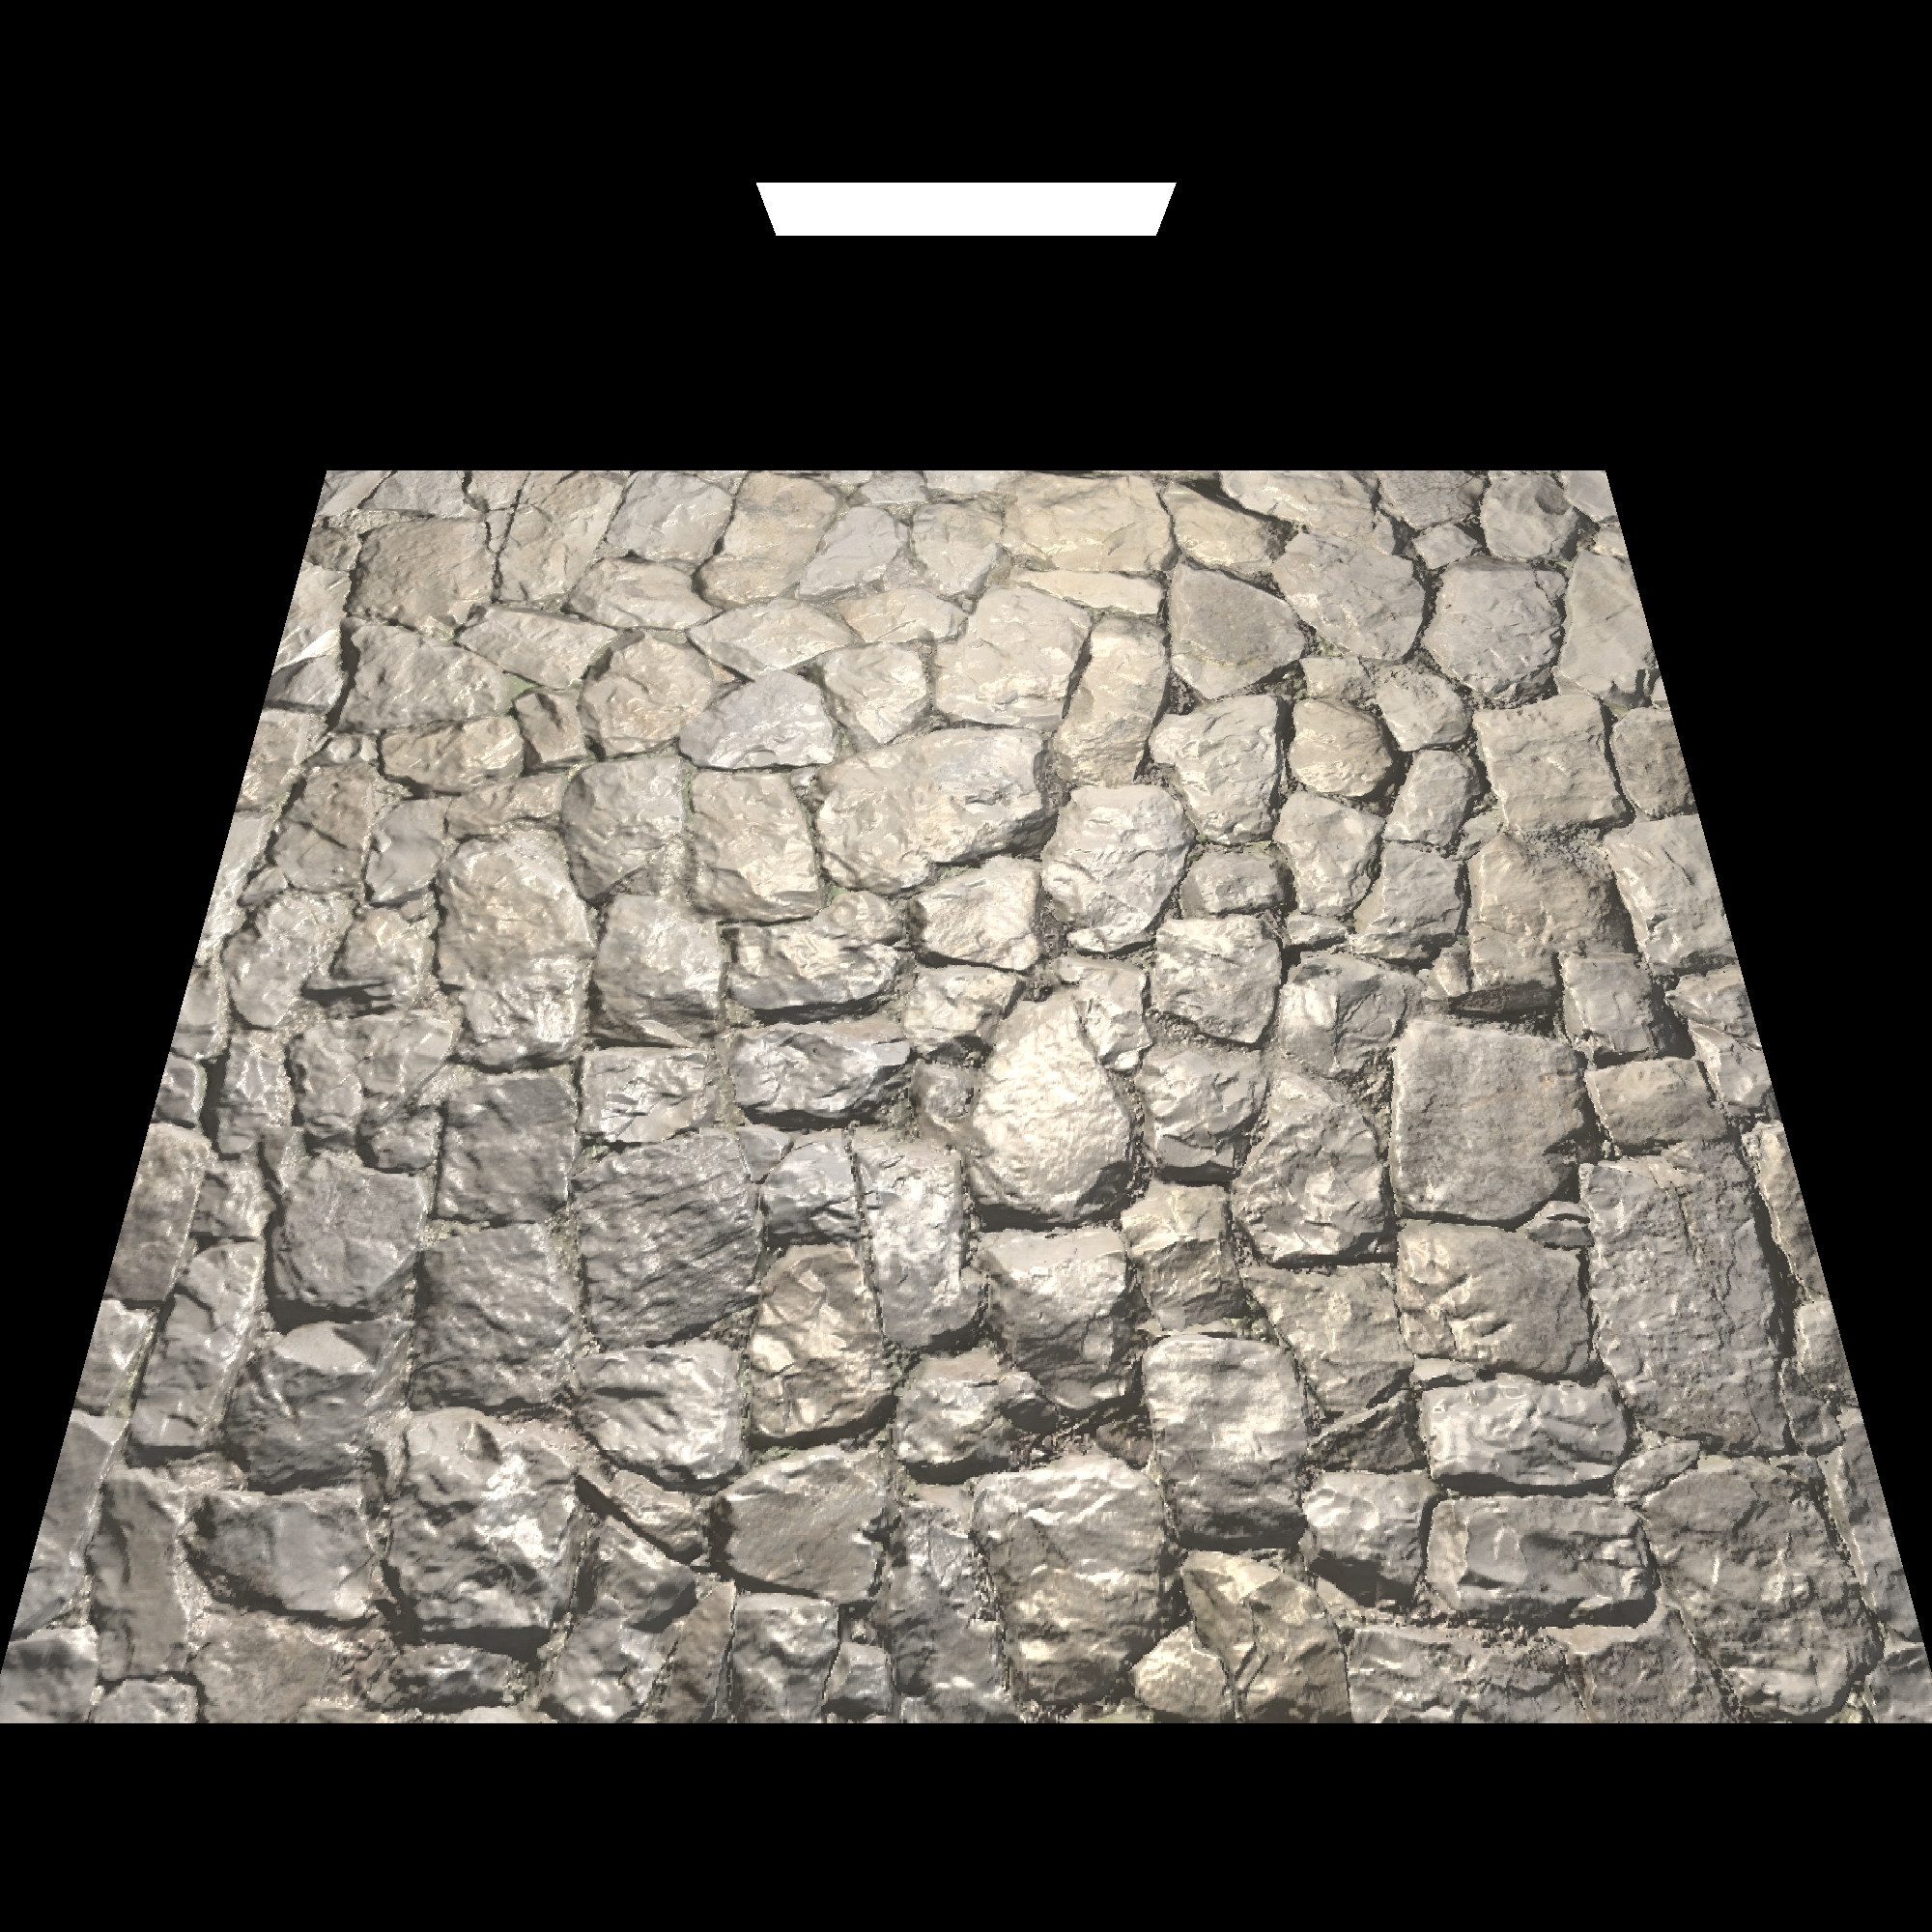
\includegraphics[width=0.45\textwidth]{"/home/lee/Desktop/CG/PA3/report/images/only_normal.png"}
		\caption{only normal map}
		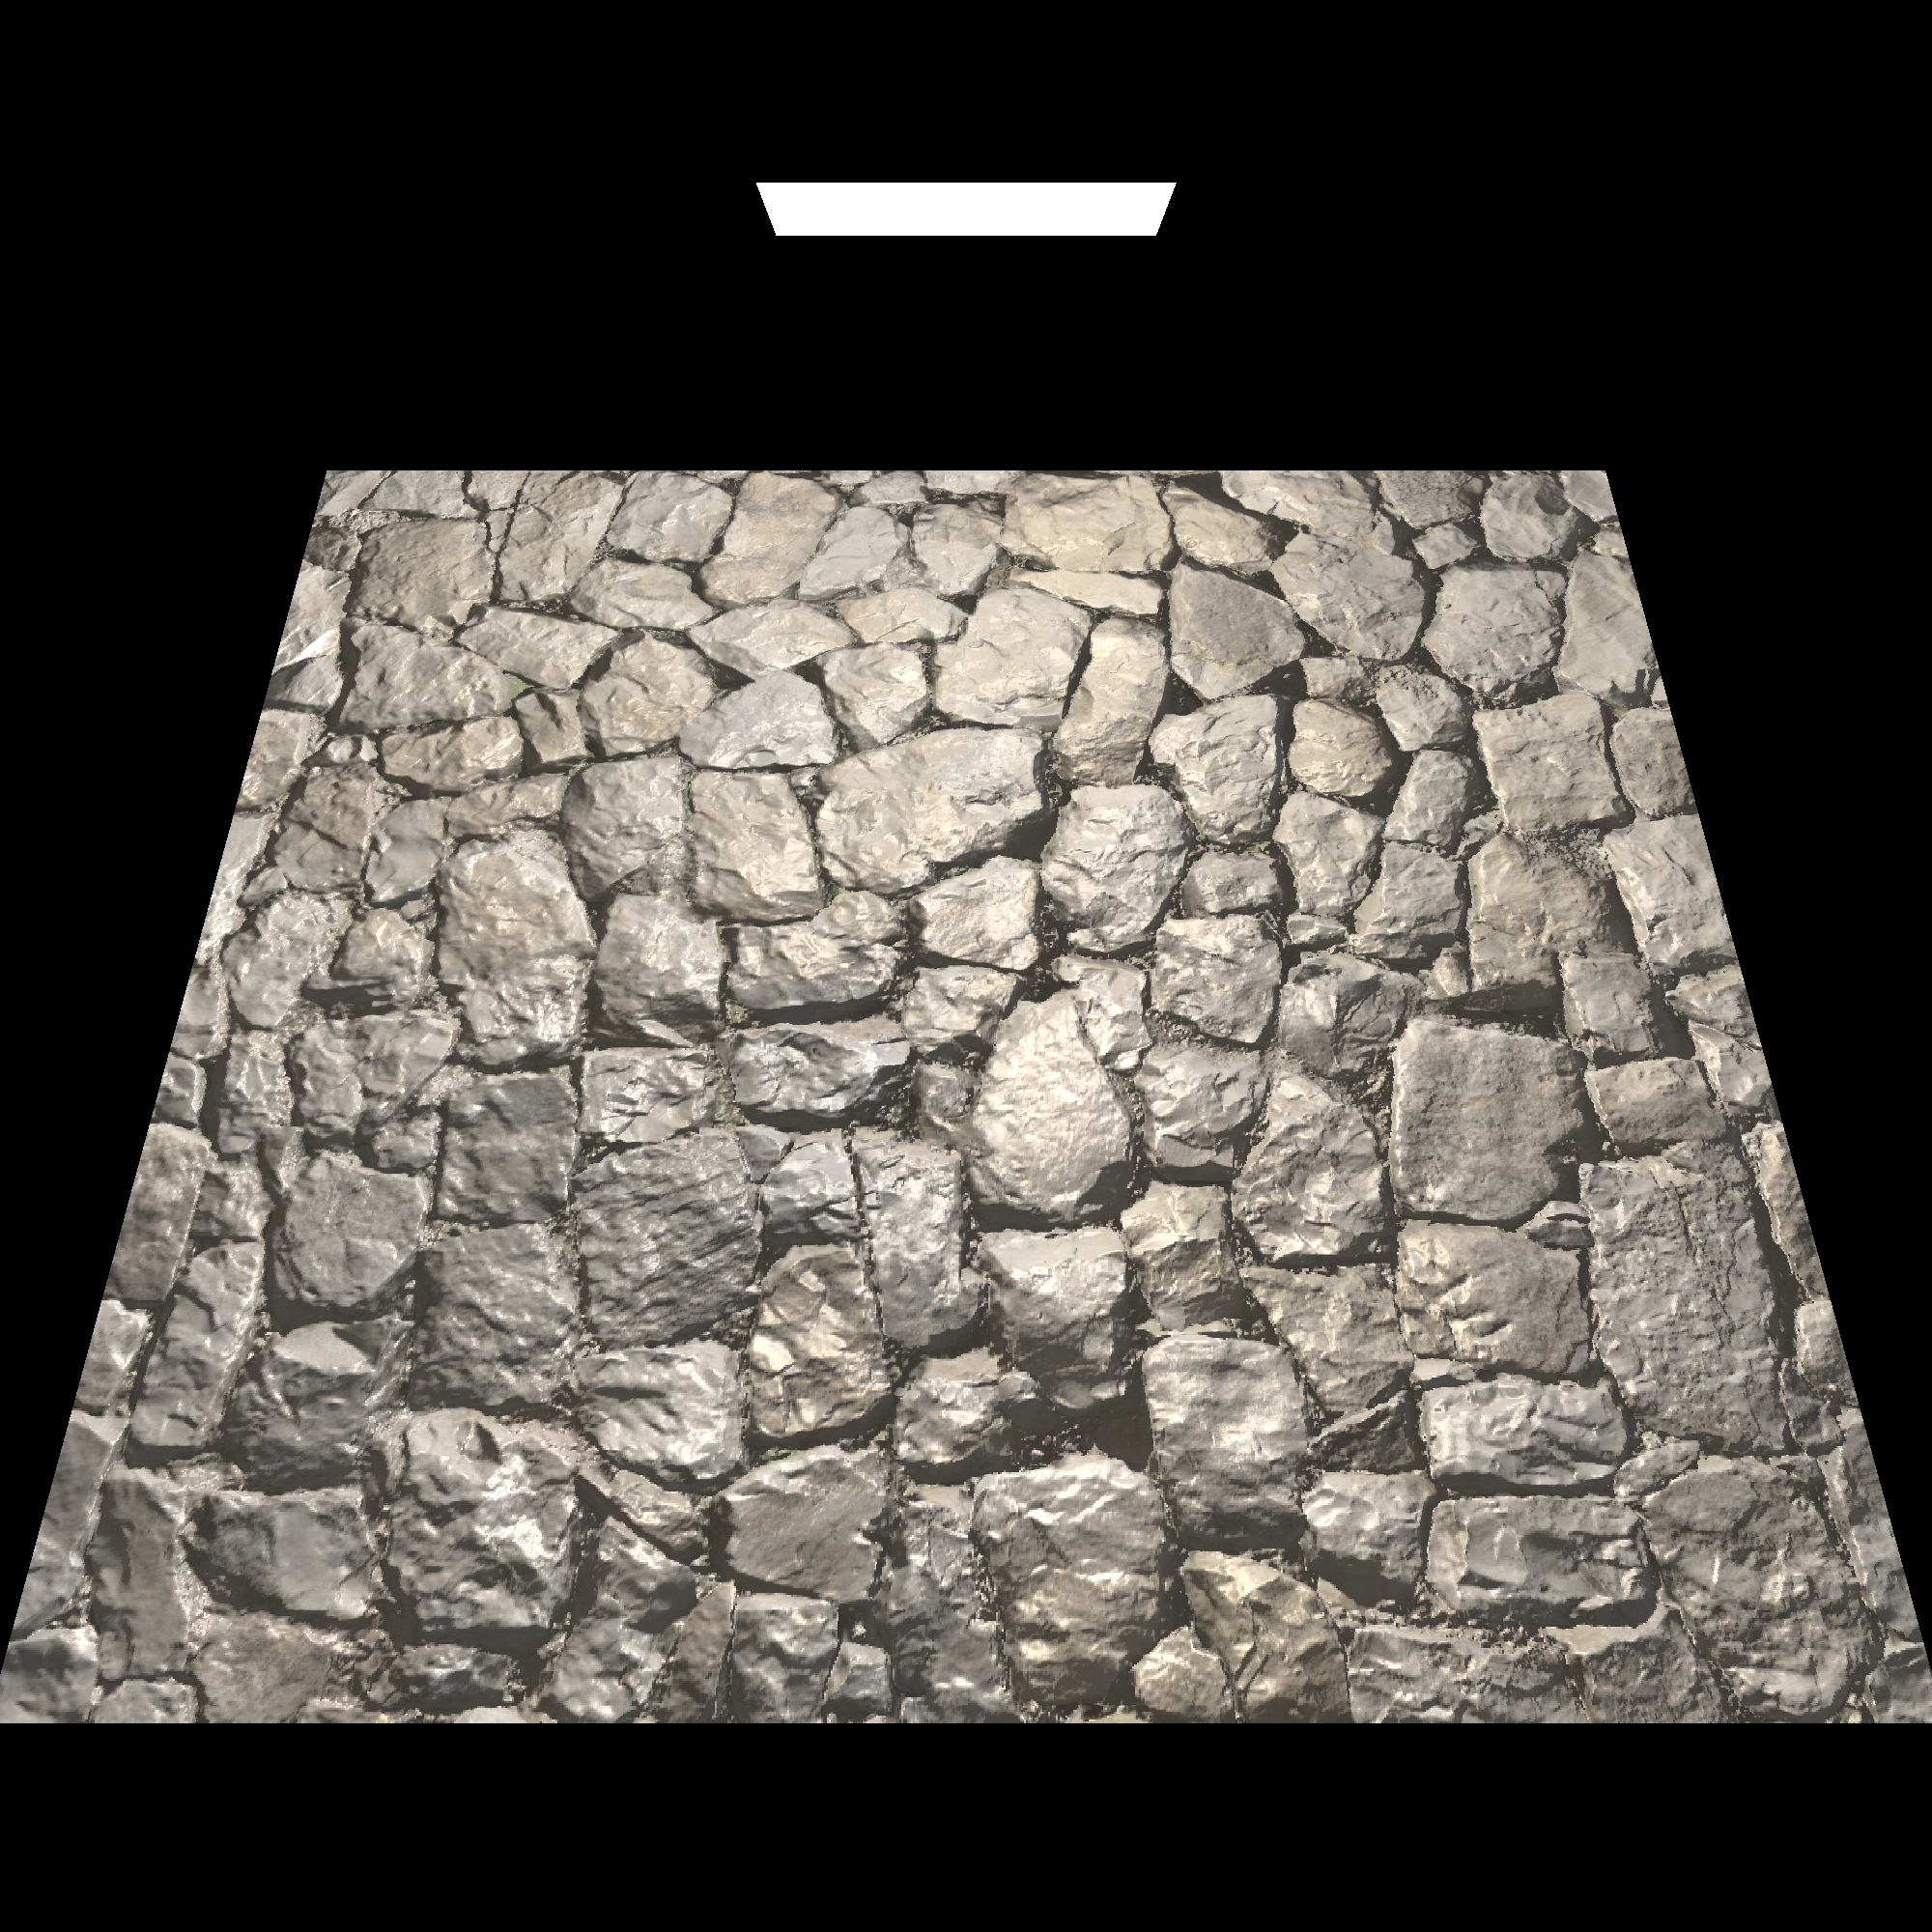
\includegraphics[width=0.45\textwidth]{"/home/lee/Desktop/CG/PA3/report/images/normal_disp.png"}
		\caption{normal + displacement map}
	\end{figure}
\end{itemize}

\end{document}
